%%%%%%%%%%%%%%%%%%%%%%%%%%%%%%%%%%%%%%%%%%%%%%%%%%%%%%%%%%%%%%%%%%%%%%%%%%%%%%%%%%%%%%
%% Author:      Nils Weber and Maximilian Stiefel
%% Date:        23.12.2017
%% University:  Uppsala Universitet
%% Department:  Institutionen för informationsteknologi 
%% Course:      Embedded Control System Project
%% Project:     PRECISELY CONTROLLED DIY ETCHING MACHINE 
%%				FOR USAGE AT HOME AND IN SMALL LABS
%%%%%%%%%%%%%%%%%%%%%%%%%%%%%%%%%%%%%%%%%%%%%%%%%%%%%%%%%%%%%%%%%%%%%%%%%%%%%%%%%%%%%%

\chapter{Background and Analysis}
\label{chap:background}
% Talk about papers and available technology. Also put the results of the small market analysis here. 

\section{Market analysis}
\label{sec:marketanalysis}
% Homemade: http://sfprime.net/pcb-etching/
% Market-Overview 
% Bath ~500$: https://goo.gl/8ebNsr
% UV illuminator ~400$:
% https://www.ebay.com/itm/Uv-Licht-Hartende-Maschine-Tragbare-Neue-2Kw-F/232345844072?hash=item3618e43968:g:5c0AAOSwa~BYVNiV
There are already different commercial and non-commercial solutions on the market to realize small-scale \gls{PCB} etching. To find possible problems and optimization potential, in order to create a superior product, a small market analysis (see tab. \ref{tab:marketanalysis}) has been carried out in the in the run-up to the development phase of the project. 

\begin{table}[H]
\centering 
\begin{tabular}{p{0.25\textwidth} p{0.2\textwidth} p{0.15\textwidth} 
p{0.35\textwidth} } 
\textbf{Product}&
\textbf{Distributor / Manufacturer}&
\textbf{Price}& 
\textbf{Technical Data}\\\hline

\specialcell[t]{
AETZGERAET 1\\
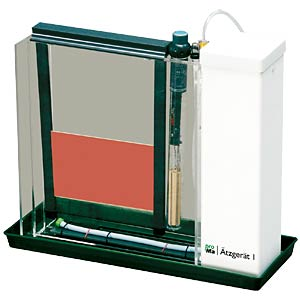
\includegraphics[width=0.15\textwidth]{./fig/etching_machine_2}
}&
Reichelt / PROMA&
129.50 EUR (03.01.2018)&
Needed Acid Volume: 1.75 l. Max. PCB Size: 235 mm x 170 mm. Heating Power: 100 W. Air Pumping System included.\\ 

\specialcell[t]{
500-004 Universal Tank\\
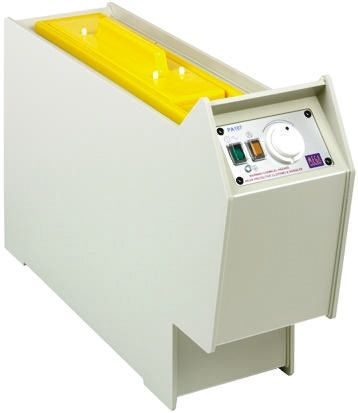
\includegraphics[width=0.15\textwidth]{./fig/etching_machine_1}
}&
RS Components / Mega Electronics&
234.26 GBP (03.01.2018)&
Needed Acid Volume: 5 l. Max. PCB Size: 315 mm x 260 mm. Air Pumping System included\\\hline

\specialcell[t]{
UV-BELICHTER 1\\
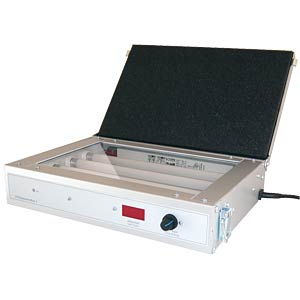
\includegraphics[width=0.15\textwidth]{./fig/uv_light_1}
}&
Reichelt / PROMA&
219.7 EUR (03.01.2018)&
Timer included (0 - 100 min). Max. PCB Size: 160 mm x 250 mm. 4 x 8 W \gls{UV} tubes. Aluminium housing.\\

\specialcell[t]{
UV Exposure Unit\\
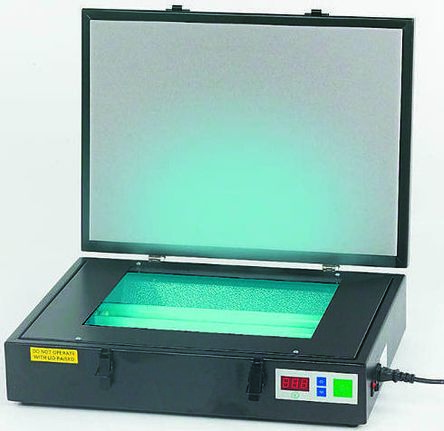
\includegraphics[width=0.15\textwidth]{./fig/uv_light_2}
}&
RS Components / Mega Electronics&
183.32 GBP (03.01.2018)&
Timer included (0 - 6 min). Max. PCB Size: 150 mm x 245 mm. 2 x 8 W \gls{UV} tubes. Metal housing.\\

\hline
\end{tabular}
\caption{Market analysis.}
\label{tab:marketanalysis}
\end{table}

Talking about the etching machines, it is a fact, that all of them do have a heater and some sort of pump to accelerate the chemical reaction introduced in chapter \ref{chap:introduction}. 
\newpar
The \myemph{500-004 Universal Tank} from \myemph{RS Components} is quite big, usually too big for small scale production. For the etching process with sodium persulfate one uses \SI{220}{\gram\per\litre} with \SI{45}{\celsius} (cf. \cite{online:aetzen}). Using the tank from RS Components one needs \SI{1.1}{\kilo\gram} of sodium persulfate, which is neither really practical nor cheap, in case one only wants to etch a few \glspl{PCB} to e.g. test a microstrip bandpass filter. Nevertheless, the design looks really robust and justifies somehow the tough price. Also the maximum \gls{PCB} size is enormous or rather a bit too big for prototyping.
\newpar
The \myemph{AETZGERAET 1} from \myemph{Reichelt} has a way more competitive price, than its equivalent from \myemph{RS Components}. It also seems to be a bit more bodge. The maximum \gls{PCB} size is still impressive as well as the heater power. 
\newpar
Presumably, there is not really a sophisticated control mechanism keeping the temperature close to the setpoint. As far as one can derive this from the given technical data, the thermostats of both devices are based on a bimetal.
\newpar
The \gls{UV} lights are both functioning with \gls{UV} fluorescent tubes. Fluorescent tubes are considered hazardous as they contain mercury vapor, which is extremely toxic (cf. \cite{online:tubes}). For this reason there are plans to ban them in the European Union. It also seems, that one pays for the \gls{UV} light power (number of tubes).
\newpar
Both \gls{UV} light exposure machines have a timer to set the exposure time. This is clearly an important and necessary feature for such a machine as the development process parameters define the quality of the final etched result. Hence, the \gls{UV} light exposure time is an important factor to fine tune the etching result. 
\newpar
Two features neither the \myemph{UV Exposure Unit} from \myemph{RS Components} nor the \myemph{UV-BELICHTER 1} have: It is not possible to adjust the light intensity and the light does only come from one direction at a time. The second shortcoming can introduce problems, since one has to turn on the light, turn it off, turn the \gls{PCB} around and repeat the exposure process. Worst-case, this might lead to alignment problems (e.g. a mounting hole on one side does not align with a mounting hole on the other side). 
\newpar
The exposure units are both relatively pricey, which might be related to the metal housing. 
\newpar
To summarize one can name some ideas how to rectify shortcomings of the currently available products for prototype \gls{PCB} etching: 
\begin{itemize}
\item The etching tank shall not be bigger than \SI{2}{\litre}, as one needs more etching liquid, which is unnecessary for small-scale production. 
\item No expensive metal housings. 
\item It shall be possible, that the user or replicator picks the heater and the compressor for air bubbles flexibly. 
\item No mercury. 
\item Double-sided \gls{UV} light exposure.
\item Precisely controlled light intensity. 
\item Digital and elegant user interface. 
\end{itemize}

\section{LED Drivers}
\label{sec:leddrivers}

\subsection{Buck Converters}
\label{subsec:buck_conv}

\begin{figure}[H]                                                         
\centering          
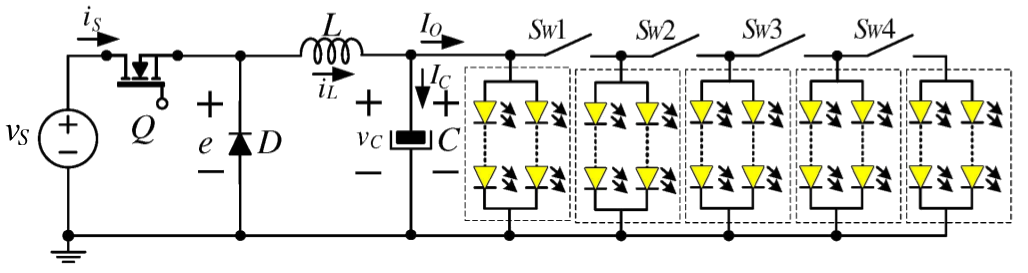
\includegraphics[width=0.7\textwidth]{./fig/buck1}   
\caption[Typcial buck converter as it can be found in a car.]{Typcial buck converter as it can be found in a car. Source: \cite{conference:buck1}.}   
\label{fig:buck1}                                                       
\end{figure}  

One of the ideas for improvements mentioned in section \ref{sec:marketanalysis} induces the use of \glspl{LED}. Therefore, in this section different state-of-the-art \gls{LED} driving techniques are introduced. To drive one \gls{LED} or a string of \glspl{LED} coupled in series one needs to keep the current constant for achieving constant light intensity. It is a well-known fact, that every single \gls{LED} differs concerning its electrical characteristics. The input to output transmission behavior i.e. \ensuremath{I(U)} differs from \gls{LED} to \gls{LED}. This is one challenge one has to master building a \gls{LED} driver. 
\newpar
A common approach, which is popular in automotive applications is a \myemph{buck converter} (cf. \cite{conference:buck1}). \myemph{Buck converters} leverage a switching-frequency to convert a high voltage into a lower voltage. In fig. \ref{fig:buck1} one can see, that in a car the current, which is drawn by the source can change rapidly, as for instance a rear light or an indicator is switched on. For this reason, a controller is needed to ensure, that enough current is provided even if rear light and indicator are switched on simultaneously. Buck converters are that popular because of their remarkable efficiency (greater than 90 \% is normal).
\newpar 
A buck converter from an electrical point of view switches between two states i.e. transistor \myemph{Q} is conducting (1) or non-conducting (2): 
\begin{enumerate}
\item If \myemph{Q} conducts \myemph{L} is directly connected to the voltage source. \myemph{C} and the load is connected to \myemph{L}. The energy stored in \myemph{L} increases. The current change results in a voltage across \myemph{L}, that counteracts the voltage of the source. This of course reduces the voltage over the load. 
\item If \myemph{Q} does not conduct \myemph{D} becomes conductive, because \myemph{L} is now a voltage source. The energy stored in the coil provides a current through the load. \myemph{L} discharges and the voltage across \myemph{L} drops again. The current through the load is still maintained. \myemph{C} helps to keep voltage and current through the load stable (close to \gls{DC} although a certain ripple is normal).  
\end{enumerate}
If the coil is charged and discharged quickly enough one can get into a steady state, where the output is within a certain range. The voltage is ramping up to a maximum and ramping down to a minimum. The output and possible input filters take care of converting this signal to a \gls{DC} signal. 
\newpar
One can also see the buck converter as a low-pass filter connected to a source with a square wave signal. The low-pass filter has ideally a cut-off frequency very close to \SI{0}{\Hz}. The filter excitation happens with a \gls{PWM} signal. One can easily explain how the steering of the current or voltage respectively works looking at the Fourier transformation of a rectangular pulse with a pulse width of \ensuremath{2\,t_0}. The pulse is defined as 
\begin{equation}
    x(t) = \begin{cases}
               1               & -t_0 \leq t \leq t_0\\
               0               & \text{otherwise}
           \end{cases}
\end{equation}
This function can be brought into the frequency domain using the most known equation of the heritage of Joseph Fourier. 
\begin{equation}
X(\omega) = \int_{-\infty}^{\infty} x(t) \cdot e^{-j \omega t} = \int_{-t_0}^{t_0} 1 \cdot e^{-j \omega t}
\end{equation}
Using \ensuremath{\int e^{at} = \frac{1}{a} e^{at}} leads to 
\begin{equation}
X(\omega) = \frac{1}{-j \omega} \, \bigl[ e^{-j \omega t_0} -  e^{j \omega t} \bigr] \text{ .}
\end{equation}
As the next step Euler's formula can be applied.
\begin{equation}
X(\omega) = \frac{2 sin(\omega t_0)}{\omega}  = \frac{2 t_0}{\omega} \frac{sin(\omega t_0)}{\omega t_0} = 2 si(\omega t_0)
\end{equation}
So what one ends up with the sinc function. As one tries to filter out every frequency except of \SI{0}{\Hz}, one can take a close look at \ensuremath{\omega = 0} with the help of l'H\^{o}spital's rule. 
\begin{equation}
\lim_{\omega \to 0} X(\omega) = \lim_{\omega \to 0} \frac{2 sin(\omega t_0)}{\omega} = \lim_{\omega \to 0} 2\,t_0\,cos(\omega t_0) = 2\,t_0  
\end{equation}
Hence, the absolute value of \ensuremath{X(\omega = 0)} becomes larger if the pulse length \ensuremath{t_0} becomes wider. This is why \gls{PWM} steering works. 

\begin{figure}[H]                                                         
\centering          
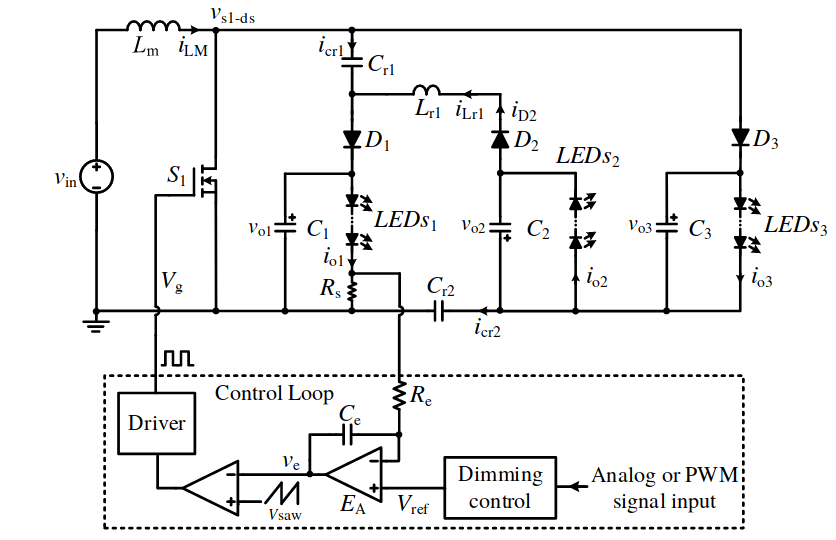
\includegraphics[width=0.7\textwidth]{./fig/buck2}   
\caption[More complex buck converter for automotive applications with analog control circuit.]{More complex buck converter for automotive applications with analog control circuit. Source: \cite{article:buck2}.}   
\label{fig:buck2}                                                       
\end{figure}  

In fig. \ref{fig:buck2} one can see a more complex draft of a buck converter with a analog controller. This circuit originates from \cite{article:buck2}. The first amplifier of the controller is an integrator. It adds memory to the control circuit. It also achieves, that the steering signal is somewhat proportional to the setpoint, which is what one can see analyzing the behavior: 
\begin{equation}
	V_e = - \frac{V_{ref}}{C_e R_e} \int V_{in} \, dt + A 
\end{equation}
whereas \ensuremath{A} is some constant. \ensuremath{V_{in} = R_s \cdot i_{o1}} is according to Ohm's law proportional to the current through the load (and a shunt resistor). The output of the first amplifier is fed into the second stage, a comparator. It compares the input with a sawtooth signal, which results in a \gls{PWM} with a duty cycle depending on the output of the first integrator. As the circuit analysis shows one deals with a proportional-integral controller here.   
\newpar 
Despite their tremendously superior efficiency, there are some disadvantages with buck converters like the switching frequency, that can cause \gls{EMI} problems. Comparing the different possibilities of buck converters one thing also becomes quite clear: Buck converters are complex. Moreover, they always need magnetic devices. Hence, designs become bulkier, less tightly integrated and more expensive if buck converters are used unnecessarily in places where they do not belong. For this reasons, linear regulators still have the right of existence nowadays. 

\subsection{Linear Regulators}
\label{subsec:buck_conv}

\begin{figure}[H]                                                         
\centering          
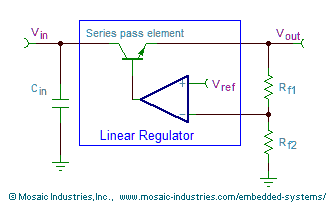
\includegraphics[width=0.4\textwidth]{./fig/linreg1}   
\caption[Typical linear regulator circuit.]{Typical linear regulator circuit. Source: \cite{online:linreg1}.}   
\label{fig:linreg1}
\end{figure}  

The other class of \gls{LED} drivers (power regulators) are linear regulators, which simply adjust their resistance in order to provide a constant current or voltage respectively. Unfortunately, a resistor converts electrical energy into heat, which is why linear regulators suffer from inefficiency, yet, they are very simple and one gets rid of possible \gls{EMI} problems caused by the switching frequency, that buck converters need. In fig. \ref{fig:linreg1} one can see a typical circuit of a linear regulator to provide a fixed voltage for a varying load impedance. This is a pure proportional controller.  

\section{Temperature Control}
\label{sec:temperatureControl}
Two approaches have been considered. Resources here can be money and time spent during development or operation.
\begin{enumerate}
\item Put more resources in sensors and save resources in the system model.
\item Put more resources in the controller model put save resources for sensors.
\end{enumerate}
The first approach was largely inspired by \cite{article:revLag}, where the application of the reversed lag principles are discussed for on-off control. A typical on-off control would result in cyclic temperature fluctuations like shown in fig. \ref{fig:waveforms}.

\begin{figure}[H]
\centering          
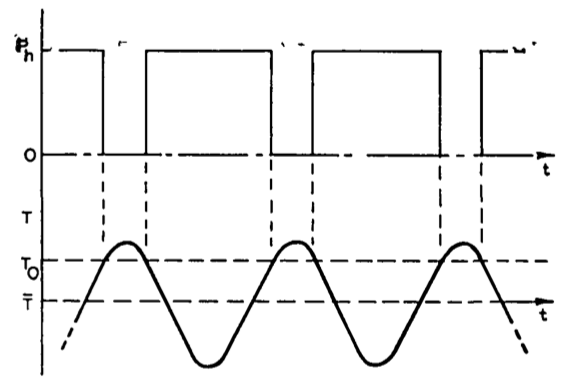
\includegraphics[width=0.4\textwidth]{./fig/waveforms} \caption[Waveforms of heating power and temperature of a system with on-off control.]{Waveforms of heating power and temperature of a system with on-off control. Source: \cite{article:revLag}.}   
\label{fig:waveforms}
\end{figure}  

The paper shows that such a system can be improved by using two control elements which are completely immersed in the fluid of the enclosure. Thus, they are not affected by different errors. One of the two output signals has to have a lagging phase angle, which can be achieved by enclosing it "within a structure which ensures that its mean temperature is that of the fluid, but thermal transmission through the structure introduces a phase lag into the fluctuating component of the temperature of the element" \cite{article:revLag}. However, the circuitry of both sensors results in a leading phase angle of the enclosed sensor with respect to the directly immersed sensor. Thus, the next temperature can be "forseen" without the need of a system model. The paper concludes that "the principle of reversed lag can be applied to an on-off temperature-control system with useful but not spectacular reductions in the amplitude of the cyclic fluctuation in temperature" \cite{article:revLag}. Furthermore, two sensors would need to be purchased to acquire essentially the same data point, which spends more resources and thus contradicts the idea of a low-cost \gls{DIY} solution for small labs or at home.
\newpar
On-off controllers are known for their energy efficiency of their output systems, compared to amplifiers. That is especially true for high power control signals. Electro-heating systems, like the here considered system, are an example for such a system, which is characterized by large time constants. That lowers the need for high frequencies to keep proper parameters of the controlled signal further. The system's dynamics can be approximated with the following equation, where, \(k\) is the static gain, \(L\) is the time delay constant and \(T\) is the system time constant \cite{article:onoffPLC}.
\begin{align}
G(s)=\frac{ke^{-sL}}{1+sT}
\end{align}
A simple on-off controller leaves an static error, which can be reduced by increase of the controller hysteresis. However, this results in increasing the amplitude and period of the oscillation of the controlled signal. This is the disadvantage of this approach. 

The paper \cite{article:onoffPLC} further introduces an inertia corrector, to counteract the described disadvantage. "The hysteresis \(h\) of the controller is the only parameter that can affect the control quality in the basic control system." The new system model with inertia correction is shown in fig. \ref{fig:inertiaCorrection}. If the time constant of the inertia correction is much smaller than the time constant of the system, "then the controller with connected corrector exhibits features of proportional-derivative controller relative to the mean value of controlled signal" \cite{article:onoffPLC}.

\begin{figure}[H]
\centering          
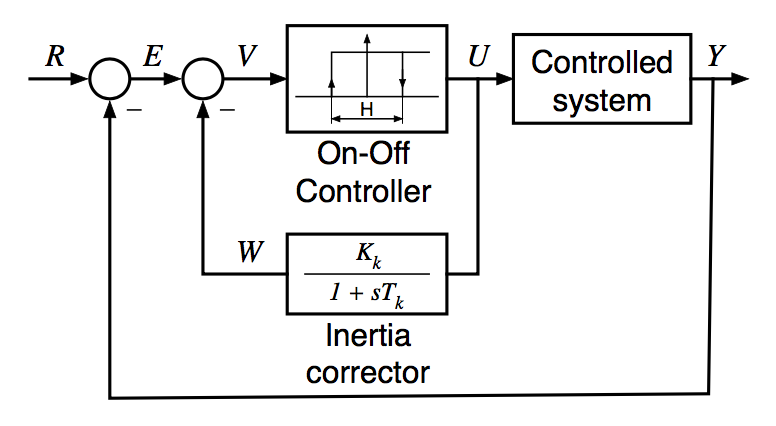
\includegraphics[width=0.4\textwidth]{./fig/inertiaCorrection} \caption[The control system with unity negative feedback and inertia corrector.]{The control system with unity negative feedback and inertia corrector. Source: \cite{article:onoffPLC}.} 
\label{fig:inertiaCorrection}
\end{figure}  

However, as the authors of \cite{article:onoffPLC} show, the steady state error can be eliminated by using an additional corrector, instead of an integrator. This proportional corrector rescales the reference value to the range of 0 to 1, before entering the control comparator. The system has to be pre-identified, but the introduction makes the mean value of the controlled signal independent from any changes of the hysteresis \cite{article:onoffPLC}.

\begin{figure}[H]
\centering          
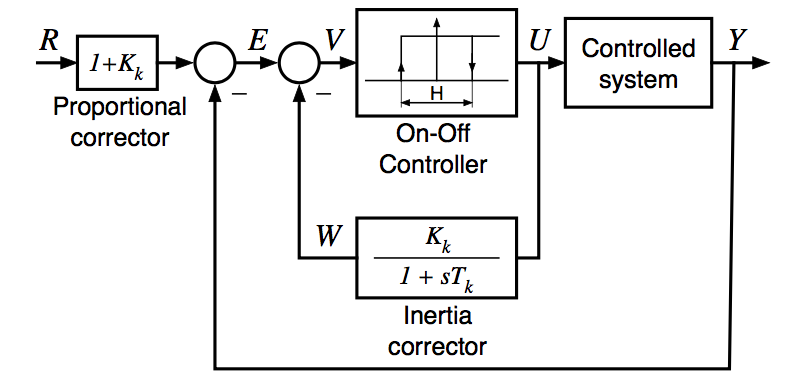
\includegraphics[width=0.4\textwidth]{./fig/inertiaCorrectionProp} \caption[The control system with proportional and inertia correctors.]{The control system with proportional and inertia correctors. Source: \cite{article:onoffPLC}.} 
\label{fig:inertiaCorrectionProp}
\end{figure} 

The paper \cite{article:onoffPLC} concludes that the introduced control system "significantly reduces an amplitude of oscillation of controlled signal and shortens its period. An additional proportional corrector eliminates an error of the mean value of the controlled signal in the steady state."